% 1988 年全国卷文科第 4 题：指数函数图象的四个选项
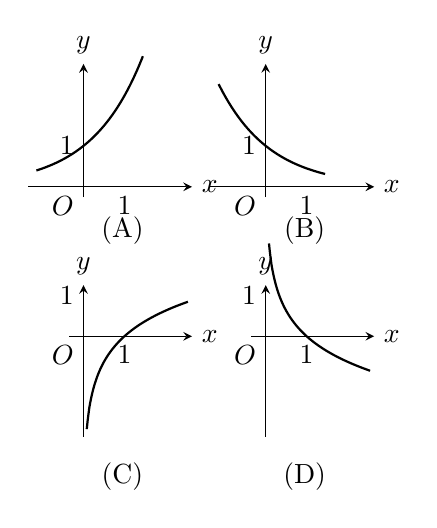
\begin{tikzpicture}[scale=0.52,>=stealth]
  \begin{scope}
    \draw[->] (-1.35,0)--(2.65,0) node[right] {$x$};
    \draw[->] (0,-0.25)--(0,3.0) node[above] {$y$};
    \draw[thick,domain=-1.15:1.45,samples=100]
      plot (\x,{exp(0.8*\x)});
    \node[left] at (0,1) {$1$};
    \node[below] at (1,0) {$1$};
    \node[below left] at (0,0) {$O$};
    \node[below] at (0.95,-0.5) {(A)};
  \end{scope}

  \begin{scope}[xshift=4.45cm]
    \draw[->] (-1.35,0)--(2.65,0) node[right] {$x$};
    \draw[->] (0,-0.25)--(0,3.0) node[above] {$y$};
    \draw[thick,domain=-1.15:1.45,samples=100]
      plot (\x,{exp(-0.8*\x)});
    \node[left] at (0,1) {$1$};
    \node[below] at (1,0) {$1$};
    \node[below left] at (0,0) {$O$};
    \node[below] at (0.95,-0.5) {(B)};
  \end{scope}

  \begin{scope}[yshift=-3.65cm]
    \draw[->] (-0.35,0)--(2.65,0) node[right] {$x$};
    \draw[->] (0,-2.45)--(0,1.25) node[above] {$y$};
    \draw[thick,domain=0.08:2.55,samples=120]
      plot (\x,{0.9*ln(\x)});
    \node[left] at (0,1) {$1$};
    \node[below] at (1,0) {$1$};
    \node[below left] at (0,0) {$O$};
    \node[below] at (0.95,-2.85) {(C)};
  \end{scope}

  \begin{scope}[xshift=4.45cm,yshift=-3.65cm]
    \draw[->] (-0.35,0)--(2.65,0) node[right] {$x$};
    \draw[->] (0,-2.45)--(0,1.25) node[above] {$y$};
    \draw[thick,domain=0.08:2.55,samples=120]
      plot (\x,{-0.9*ln(\x)});
    \node[left] at (0,1) {$1$};
    \node[below] at (1,0) {$1$};
    \node[below left] at (0,0) {$O$};
    \node[below] at (0.95,-2.85) {(D)};
  \end{scope}
\end{tikzpicture}
